\documentclass{bfh}

\usepackage[numbers]{natbib}
\usepackage{xfrac}

\title{Informatikseminar}
\subtitle{Bitmessage -- Kommunikation ohne Metadaten}
\author{Christian Basler}
\tutor{Kai Brünnler}
\date{\today}

\newcommand{\msg}[1]{\textit{\textcolor{RedOrange}{#1}}}
\newcommand{\obj}[1]{\textbf{\textcolor{OliveGreen}{#1}}}
\newcommand{\node}[1]{\textbf{\textcolor{MidnightBlue}{#1}}}

\begin{document}
  \maketitle

  \tableofcontents

  \newpage
  % Section basics
    \section{Basics}

  While encryption technology like PGP or S/MIME provides a secure way to protect content from prying eyes, we lerned from Edward Snowden that metadata - information about who communicates with whom - is equally interesting and much easier to analyze.

  With e-mail, we can only prevent this by encrypting the connection to the server as well as between servers. Therefore we can only hope that both our and the recipient's e-mail provider are both trustworthy and competent.

  With Bitmessage we send a message to a sufficiently large number of participants, with the intended recipient among them. The message is encrypted such as only the person in possesion of the private key can decrypt it. All participants try to do this in order to find their messages.

  \newpage
  \section{PyBitmessage}

  PyBitmessage ist der Standard Bitmessage Client und, wie der Name andeutet, in Python implementiert. Der Client bietet zwar alle Funktionen von Bitmessage, die User Experience ist allerdings nicht ganz optimal. Insbesondere lassen sich Nachrichten nicht in Ordner verschieben oder mit Labels versehen.

  \begin{figure}[h]
  \centering
  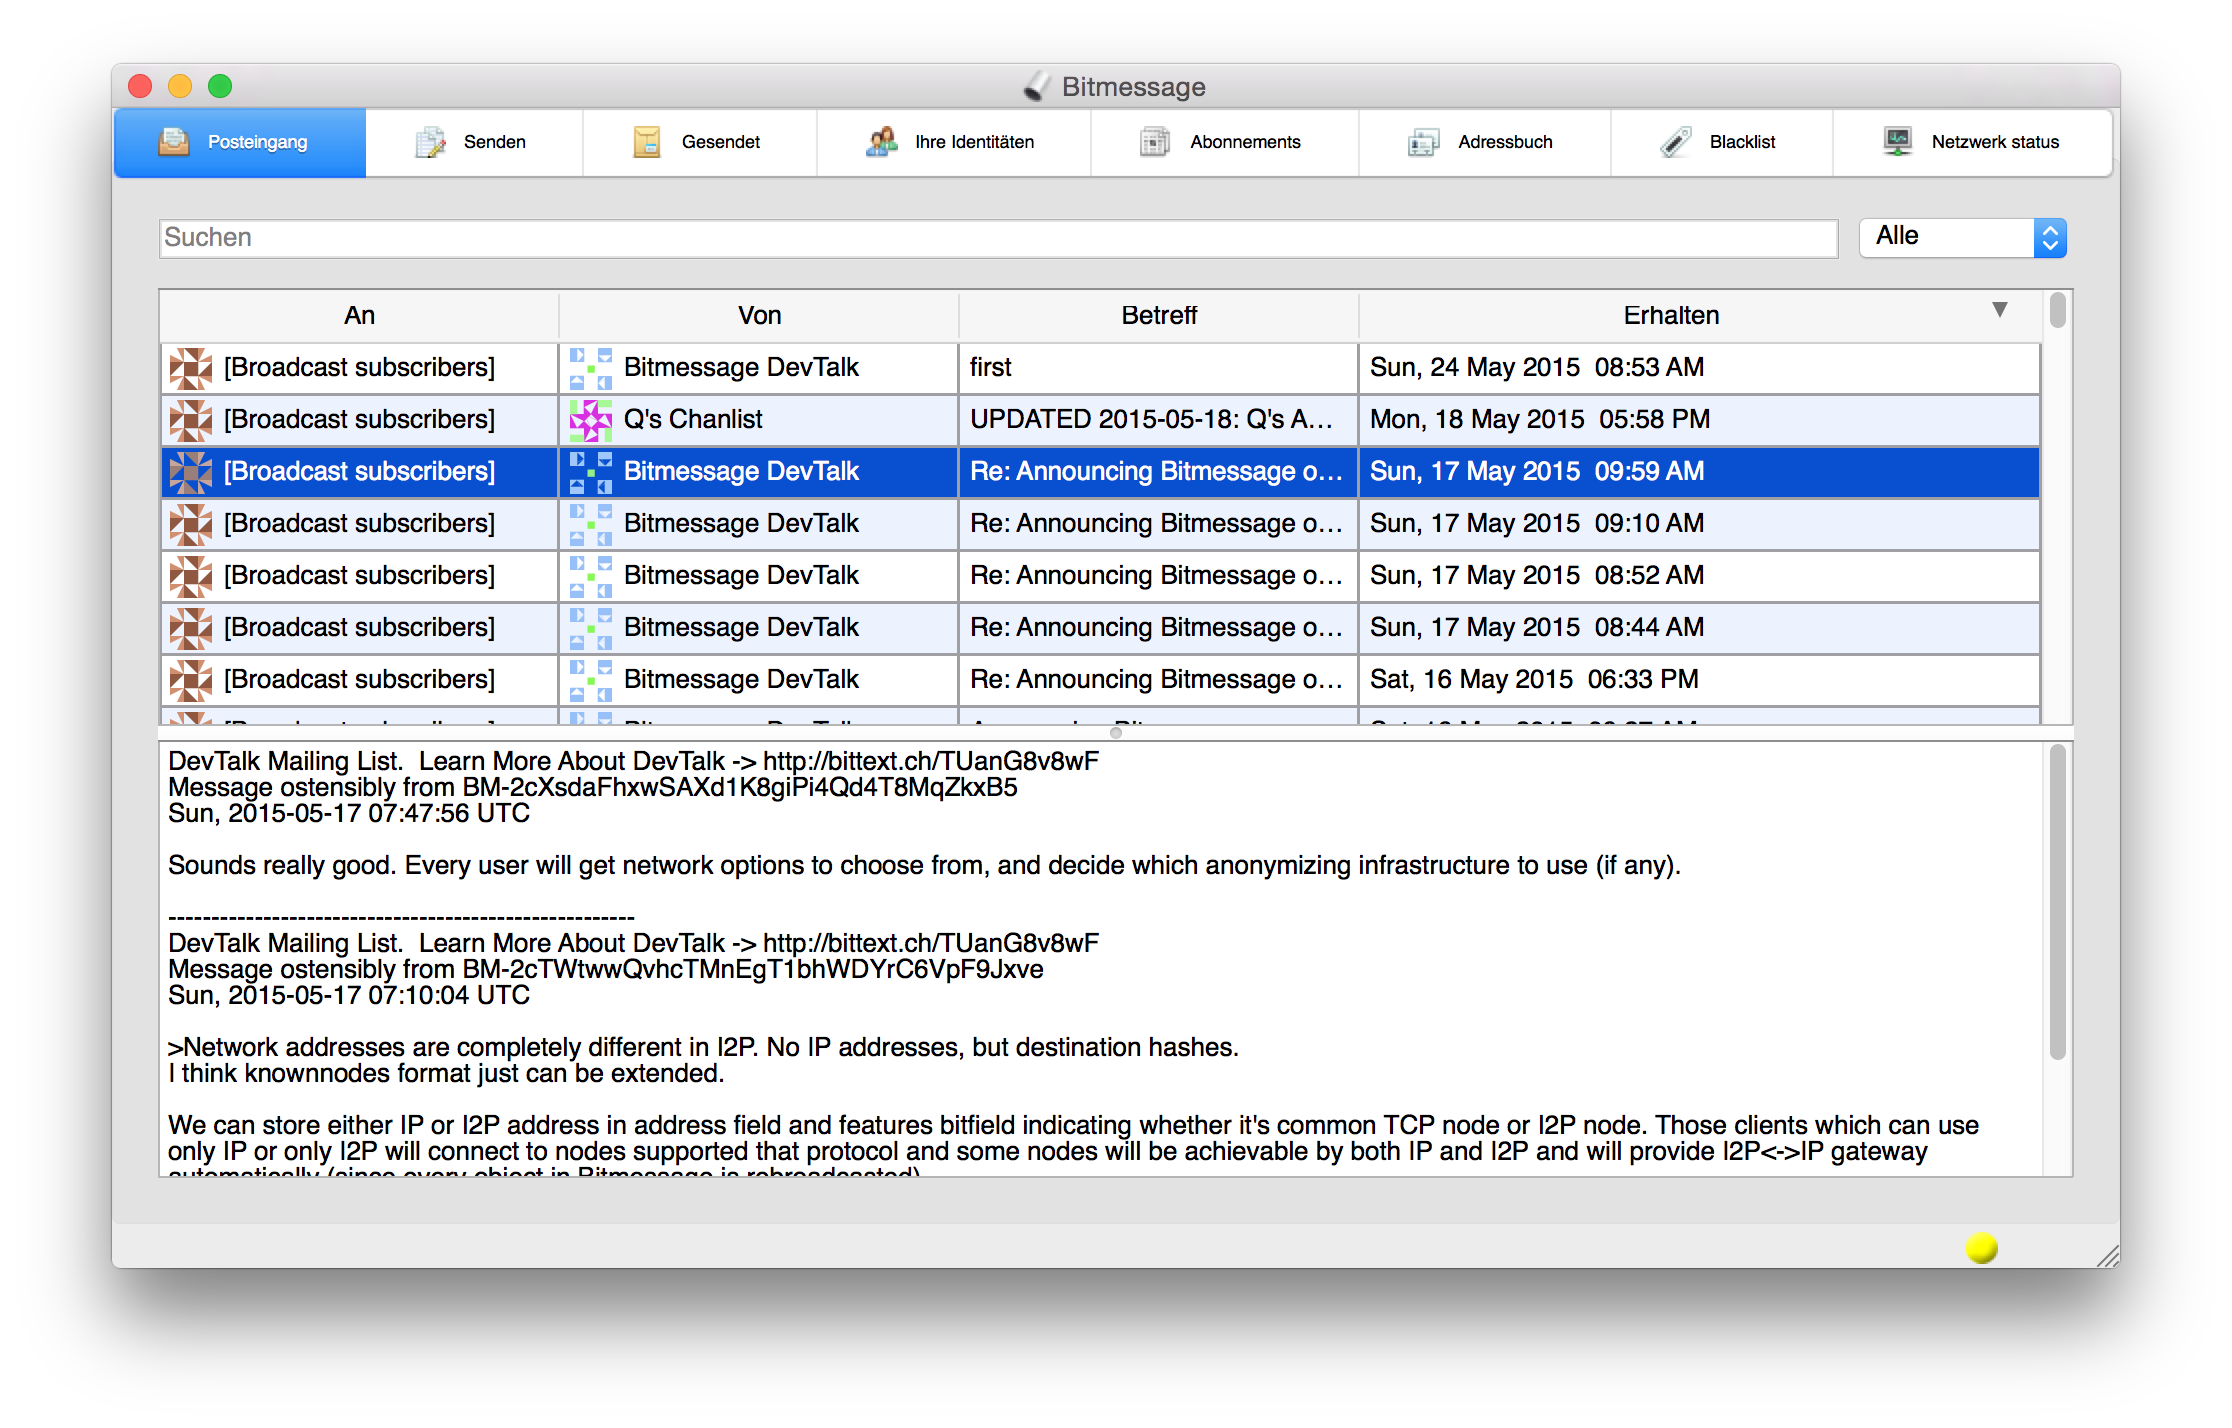
\includegraphics[width=0.8\textwidth]{images/PyBitmessage-Inbox.png}
  \caption[PyBitmessage: Inbox]{Der Posteingang von PyBitmessage.}
  \label{fig:inbox}
  \end{figure}

  Der Client ist ausserdem ziemlich langsam im Berechnen des Proof of Work. Auf einem MacBook Pro von 2012 kann es durchaus einige Minuten dauern bis eine Nachricht gesendet werden kann.

%  \begin{figure}[h]
  \begin{wrapfigure}{r}{0.5\textwidth}
  \centering
  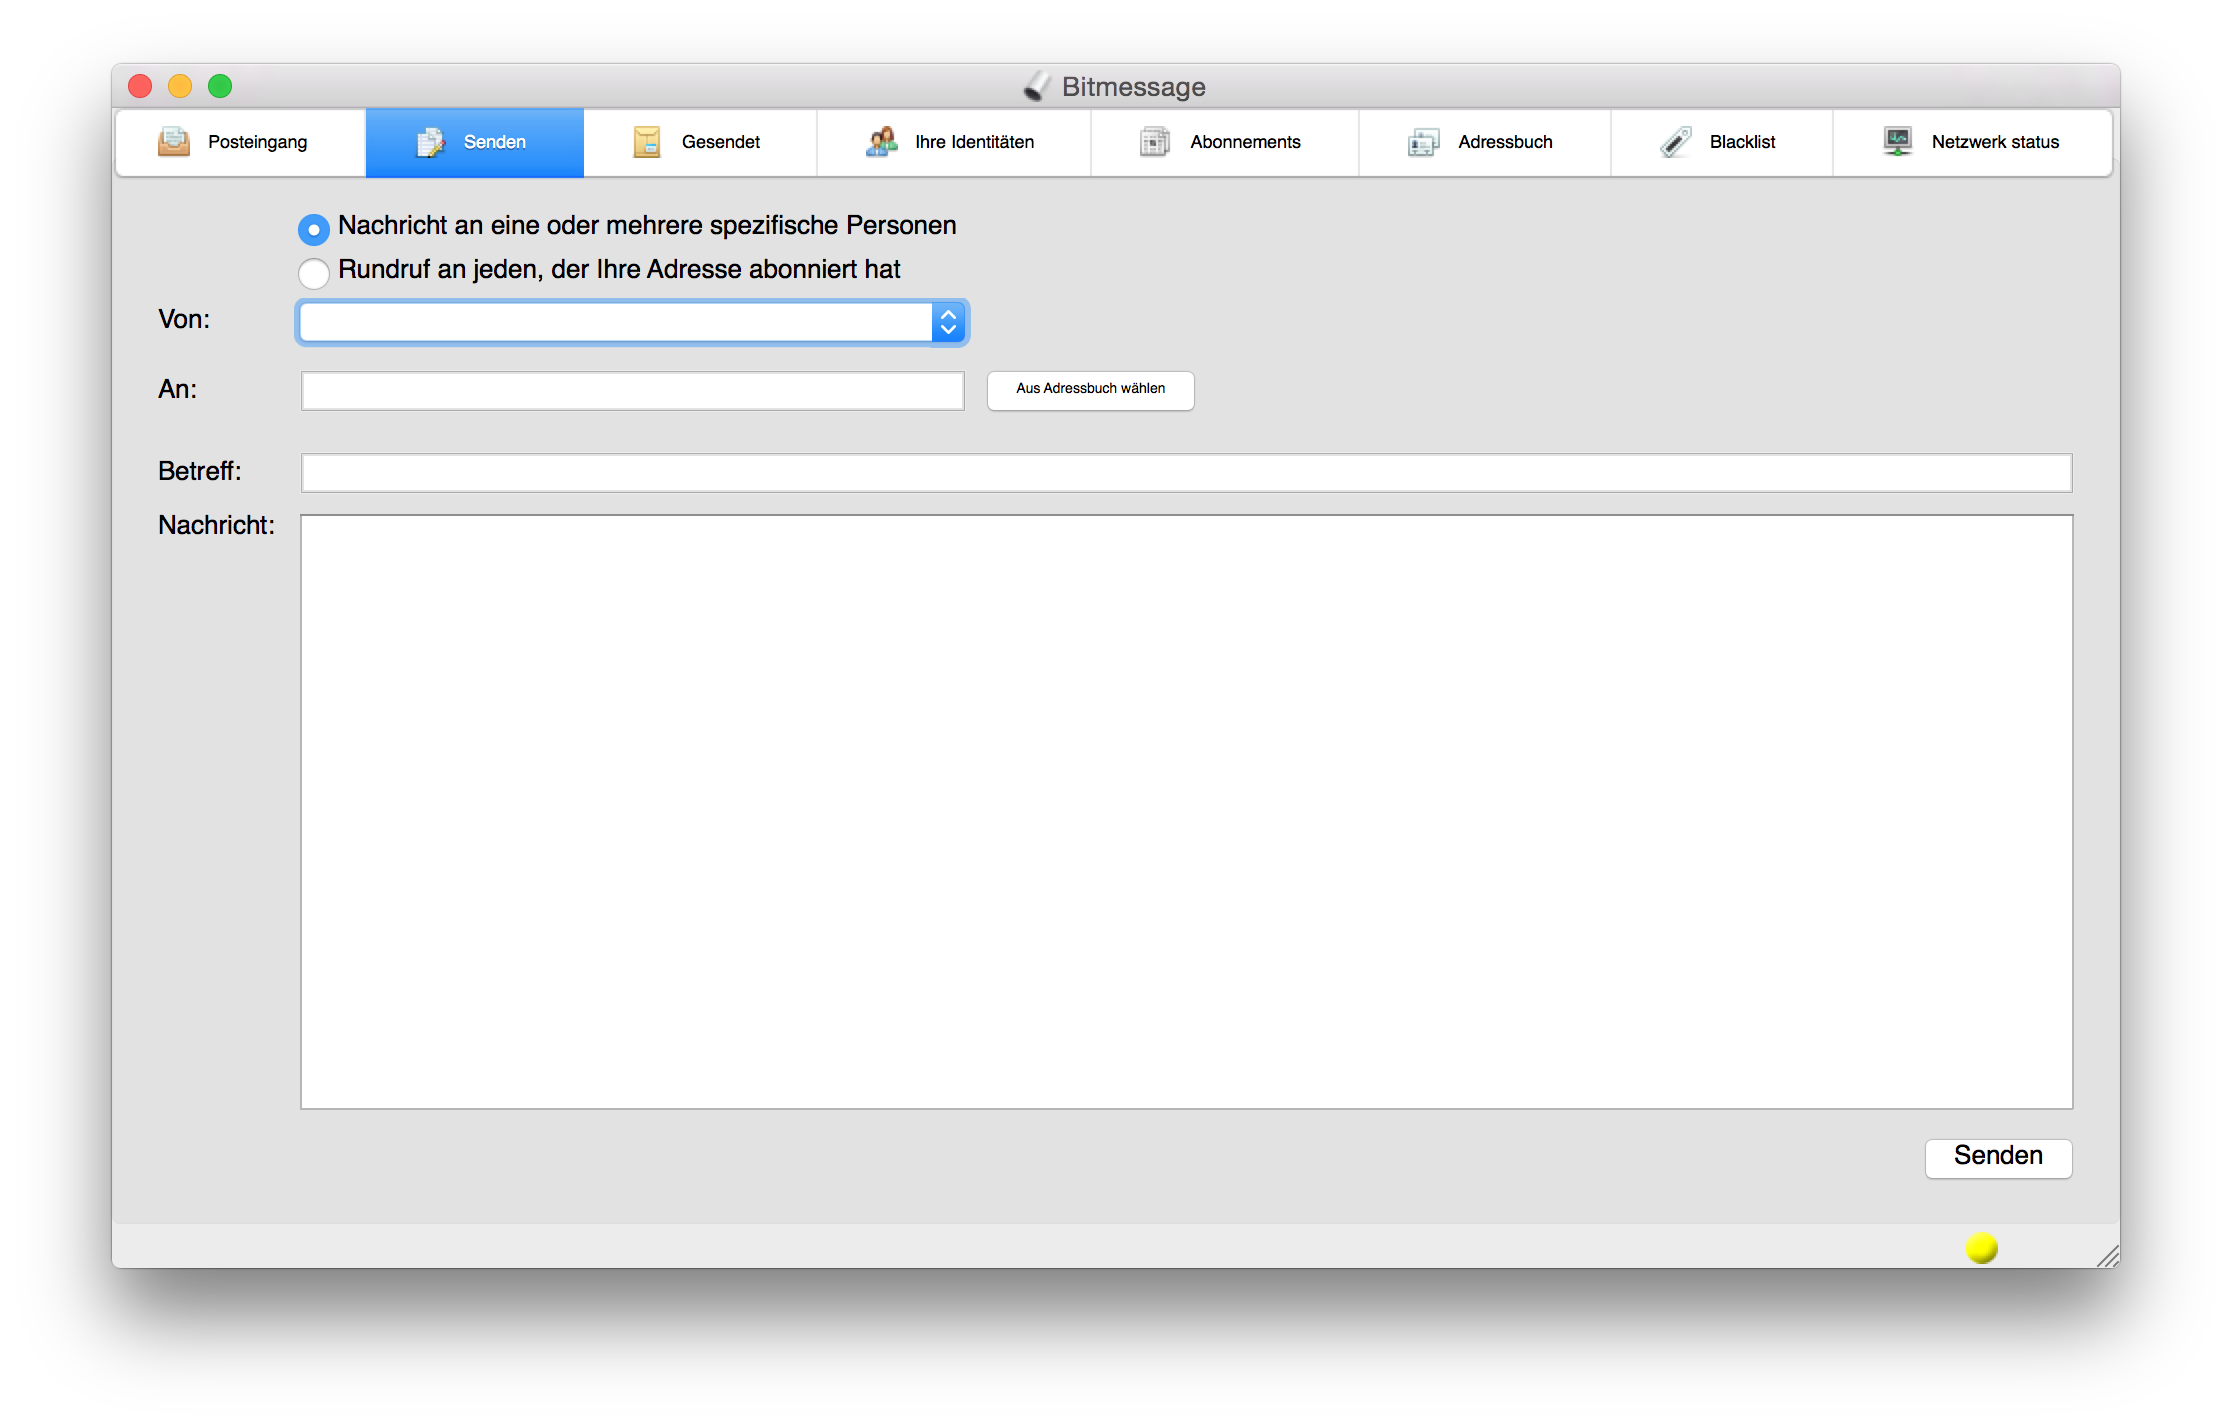
\includegraphics[width=0.5\textwidth]{images/PyBitmessage-Send.png}
  \caption[PyBitmessage: Senden]{Eine neue Nachricht erfassen.}
  \label{fig:inbox}
  \end{wrapfigure}

  Wenn man die Funktionsweise des Protokolls sieht, liegt die Idee natürlich nicht weit Meldungen an mehrere Empfänger gleichzeitig senden zu wollen. Dies geht so, dass die Adresse selbst in einen privaten Schlüssel umgewandelt wird und so zum \textit{entschlüsseln} der Broadcasts benutzt werden kann. Entsprechend kann man beim Erfassen einer Nachricht wählen ob sie an einen bestimmten Empfänger gehen soll oder an alle, die unsere Broadcasts abonniert haben. Jeder, der die Adresse kennt kann dabei allerdings die darüber gesendeten Broadcasts lesen.

  \newpage
  \section{Protokoll}

  Wir benutzen die folgende Konvention um zwischen verschiedenen Bestandteilen der Protokolls zu unterscheiden:

  \begin{tabular}{@{}>{$}l<{$}l@{}}
	\msg{version} & für Meldungen zwischen Netzwerkknoten \\
	\obj{pubkey} & für Objekte welche im Netzwerk verteilt werden \\
	\node{A} & für einzelne Netzwerkknoten \\
  \end{tabular}


  \subsection{Nomenklatur}

  Es gibt einige Begriffe welche schnell verwechselt werden können. Es folgt eine Liste der verwirrendsten.

  \subsubsection{message, msg}
  Eine Nachricht oder \msg{message} wird von einem Netzwerkknoten zum anderen geschickt, z.B. um neue Objekte anzukündigen oder um die Verbindung aufzubauen.

  Ein \obj{msg}-Objekt andererseits enthält die verschlüsselte Nachricht von einem Benutzer an einen anderen.

  \subsubsection{payload}
  Payload werden die Nutzdaten eines Protokolls genannt. Es gibt drei Arten von Payload:
  \begin{enumerate}
  \item Der Payload von Meldungen, z.B. \textit{Inventory Vectors}.
  \item Der Payload von Objekten. Dieser wird im Netzwerk verteilt.\footnote{Und ist Teil vom Meldungs-Payload.}
  \item Verschlüsselter Payload, der Chiffretext mit einigen Zusatzinformationen welche für die Entschlüsselung benötigt werden.\footnote{Dieser wiederum ist Teil vom Objekt-Payload.}
  \end{enumerate}

  \subsubsection{object}
  Ein Objekt ist eine Art Meldung, deren Payload zwischen allen Netzwerkknoten verteilt wird. Manchmal wird auch nur der Payload gemeint. Um ein Objekt zu senden, wird ein \textit{Proof of Work} benötigt.

  \subsection{Ablauf}

  Der neu gestartete Netzwerkknoten \node{A} stellt die Verbindung zu einem zufälligen Knoten \node{B} aus seinem Knotenverzeichnis her und sendet eine \msg{version}-Meldung, die die aktuellste unterstützte Protokollversion ankündigt. Falls \node{B} die Version akzeptiert,\footnote{Eine Version wird normalerweise akzeptiert, wenn sie höher oder gleich der eigenen höchsten unterstützten Version ist. Knoten, welche eine experimentelle Protokollversion implementieren, können auch ältere Versionen akzeptieren.} antwortet er mit einer \msg{verack}-Meldung, gefolgt von der eigenen \msg{version} mit ihrer neusten unterstützten Protokollversion. Knoten \node{A} entscheidet nun ob er die Version von \node{B} akzeptiert und sendet in diesem Fall seine \msg{verack}-Meldung.

  Wenn beide Knoten die Verbindung akzeptieren, senden sie je eine \msg{addr}-Meldung mit bis zu 1000 bekannten Knoten, gefolgt von einer oder mehreren \msg{inv}-Meldungen, welche alle bekannten gültigen Objekte mitteilt. Danach wird eine \msg{getdata}-Meldung für die noch fehlenden Objekte gesendet.

  Auf \msg{getdata} antwortet der Knoten mit einer \msg{object}-Meldung, welche dann das angeforderte Objekt enthält.

  Ein Knoten verbindet sich aktiv mit acht anderen Knoten und erlaubt beliebig viele eingehende Verbindungen. Wenn ein Benutzer an Knoten \node{A} ein neues Objekt erzeugt, wird es mittels \msg{inv}-Meldung bei acht der angebundenen Knoten angeboten. Diese fordern es an und bieten es wiederum bei acht Nachbarknoten an, bis es an alle Knoten verteilt ist.

  \subsection{Meldungen}

  Die Meldungen, Objekte und das Binärformat sind im Bitmessage-Wiki gut dokumentiert, die Beschreibungen hier sind deshalb darauf konzentriert um was es geht und wie man sie benutzt.\cite{wiki:protocol}

  \subsubsection{version / verack}
  Die \msg{version}-Meldung enthält die aktuellste vom Knoten unterstützte Protokollversion, die Streams für welche er sich interessiert und die unterstützten Features. Falls der andere Knoten akzeptiert, bestätigt er mittels \msg{verack}. Die Verbindung gilt als initialisiert wenn beide Knoten eine \msg{verack}-Meldung gesendet haben.

  \subsubsection{addr}
  Eine \msg{addr}-Meldung enthält bis zu 1000 bekannte Knoten mit deren IP-Adresse, Port, Stream und unterstützten Features. Die IP-Adressen werden dabei im IPv6-Format dargestellt, für IPv4-Adressen also 12 Bytes \texttt{00 00 00 00 00 00 00 00 00 00 FF FF}, gefolgt von den vier Bytes der IPv4-Adresse.

  \subsubsection{inv}
  Eine \msg{inv}-Meldung enthält die Hashes von bis zu 50000 gültigen Objekten. Falls das Inventar mehr Objekte enthält können mehrere Meldungen gesendet werden.

  \subsubsection{getdata}
  Die Meldung \msg{getdata} kann bis zu 50000 Objekte anfordern, indem es deren Hashes sendet.

  \subsubsection{object}
  Die \msg{object}-Meldung enthält ein angefordertes Objekt, das eines von folgenden sein kann:

  \listinginfo{}{getpubkey}{Eine Aufforderung an eine Adresse, deren öffentlichen Schlüssel zu senden. Dieser wird benötigt um die Meldung an diese Adressen zu verschlüsseln.}{}
  \listinginfo{}{pubkey}{Ein öffentlicher Schlüssel. Siehe \ref{subsec:addr} \nameref{subsec:addr}}{}
  \listinginfo{}{msg}{Eine Nachricht an einen bestimmten Benutzer.}{}
  \listinginfo{}{broadcast}{Eine Nachricht, welche auf eine spezielle Art verschlüsselt wird. So kann jeder, der die sendende Adresse kennt, sie entschlüsseln.}{}

  \subsubsection{ping / pong / getbiginv}
  Wer den Source Code von PyBitmessage untersucht, ist vielleicht über einige Meldungen irritiert, welche implementiert zu sein scheinen, aber nirgends in der offiziellen Spezifikation zu finden sind. \msg{Ping} bringt einen Knoten (sofern implementiert) dazu ein \msg{pong} zurückzusenden. \msg{Getbiginv} scheint dafür gedacht zu sein das ganze Inventar abzufragen. Verwendet werden diese Meldungen jedoch nirgends.\cite{issue:112}

  \subsection{Adressen}
  \label{subsec:addr}

  \textit{BM-2cXxfcSetKnbHJX2Y85rSkaVpsdNUZ5q9h}: Adressen beginnen mit "BM-"{} und sind, genau wie Bitcoin-Adressen, Base58 codiert.\footnote{Dieses verwendet die Zeichen 1-9, A-Z und a-z ohne die leicht verwechselbaren Zeichen I, l, 0 and O.}

  \listinginfo{}{version}{Adressversion. Version 1 wird vom Netzwerk nicht mehr unterstützt.}{0x02, 0x03 oder 0x04}
  \listinginfo{}{stream}{Stream-Nummer. Im Moment wird praktisch nur Stream 1 verwendet.}{0x01}
  \listinginfo{}{ripe}{Hash der aneinandergefügten öffentlichen Schlüssel zum Signieren und Verschlüsseln. Wichtig: in \obj{pubkey}-Objekten werden die Schlüssel ohne führendes 0x04 gesendet, doch um den Ripe zu berechnen muss dieses Byte vorangestellt werden. Da dies für fast alle Verwendungszwecke der Schlüssel nötig ist, lohnt es sich dies gleich beim Erstellen des Objekts zu machen.

Führende Nullen werden dabei weggelassen. Es wird ausserdem ein Schlüsselpaar gesucht, dessen Ripe mindestens eine führende Null hat.}{ripemd160(sha512(pubSigKey + pubEncKey))}
  \listinginfo{}{checksum}{Die ersten vier Bytes eines doppelten SHA-512-Hashs der vorangehenden Daten.}{sha512(sha512(version + stream + ripe))}

  \subsection{Verschlüsselung}

  Bitmessage benutzt Elliptische-Kurven-Kryptographie sowohl zum Signieren als auch zum Verschlüsseln. Die Mathematik dahinter ist ziemlich kompliziert. Sie basiert jedoch auf dem bewährten Prinzip, eine mathematische Operation durchzuführen, welche in eine Richtung relativ einfach, jedoch sehr schwierig umzukehren ist. An Stelle der sonst üblichen zwei grossen Primzahlen werden hier ein Punkt auf der elliptischen Kurve mit einer sehr grossen Zahl multipliziert.\footnote{Falls Sie wissen möchten wie das genau geht, beginnen Sie auf \url{http://de.wikipedia.org/wiki/Elliptische_Kurve} und \url{http://de.wikipedia.org/wiki/Elliptic_Curve_Cryptography}. Falls Sie etwas machen möchten das funktioniert, verwenden Sie aber lieber eine Bibliothek wie Bouncy Casle, welche die harte Arbeit übernimmt.}

  Der Vorteil von elliptischen Kurven ist einerseits, dass man keine grossen Primzahlen suchen muss, andererseits aber auch, dass die Schlüssel bei gleicher Verschlüsselungsstärke viel kürzer sein können.

  Die Benutzerin, nennen wir sie Alice, benötigt ein Schlüsselpaar, welches aus dem privaten Schlüssel
$$k$$
besteht, der eine riesige\footnote{32 Bytes} Zufallszahl darstellt, und einem öffentlichen Schlüssel
$$K = G k$$
der einen Punkt auf der vorher definierten Kurve repräsentiert.\footnote{Bitmessage benutzt eine Kurve namens \textit{secp256k1}.} Beachten Sie bitte dass dies keine einfache Multiplikation ist, sondern die skalare Multiplikation eines Punktes auf der elliptischen Kurve. $G$ ist der Startpunkt für alle Operationen auf einer spezifischen Kurve.

  Ein anderer Benutzer, Bob, kennt den öffentlichen Schlüssel. Um eine Nachricht zu verschlüsseln erstellt er das temporäre Schlüsselpaar
$$r$$
und
$$R = G r$$
Danach berechnet er
$$K r$$
benutzt den daraus folgenden Punkt um die Meldung zu verschlüsseln\footnote{Genaugenommen wird ein doppelter SHA-512-Hash über der X-Koordinate benutzt um den symmetrischen Schlüssel zu erzeugen.} und sendet $K$ zusammen mit der verschlüsselten Nachricht.

  Wenn Alice die Meldung empfängt, benutzt sie die Tatsache dass
$$K r = G k r = G r k = R k$$
also berechnet sie einfach $R k$ um die Meldung zu entschlüsseln.

  Die genaue von Bitmessage verwendete Methode wird Elliptic Curve Integrated Encryption Scheme oder ECIES genannt, welche auf Wikipedia detailliert beschrieben wird (\url{http://de.wikipedia.org/wiki/Elliptic_Curve_Integrated_Encryption_Scheme}).

  \subsubsection{Signatur}

  Um Objekte zu signieren verwendet Bitmessage Elliptic Curve Digital Signature Algorithm oder ECDSA. Dies ist etwas komplizierter als ECIES. Wenn Sie Details wissen möchten ist Wikipedia einmal mehr eine gute Anlaufstelle: \url{http://de.wikipedia.org/wiki/Elliptic_Curve_DSA}.

  Ein interessantes Detail für potentielle Entwickler von Bitmessage-Clients --- vor allem wenn Sie es mit einem objektorientierten Ansatz machen möchten: die Signatur geht über alles aus dem Objekt-Header ohne das Nonce und alles aus dem Objekt-Payload ohne die Signatur selbst. Natürlich sind nicht alle Objekte signiert und die Signatur befindet sich im verschlüsselten Teil des Objekt-Payloads.\footnote{Mein Ansatz: zuerst denken, dann falsch implementieren, dann viel umschreiben.}

  \begin{figure}[htp]
  \centering
  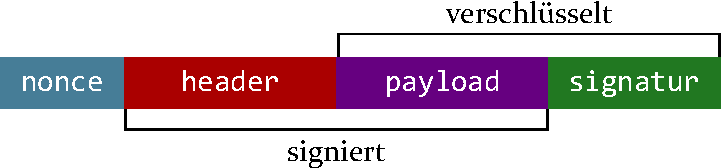
\includegraphics[width=0.7\textwidth]{images/signature.pdf}
  \caption[Signatur: Datenstruktur]{Aufbau von signierten und verschlüsselten Daten}
  \label{fig:signature}
  \end{figure}

  \newpage
  \section{Probleme}

  \subsection{Skalierbarkeit}

  Bitmessage skaliert nicht.\footnote{Noch nicht.} Gibt es sehr wenige Benutzer, so gibt es auch keine Anonymität. Mit einer kleinen Anzahl von Benutzern ist es einfach (beispielsweise für die NSA), den Verkehr zwischen Knoten zu analysieren um herauszufinden wer wem schreiben könnte.

  Mit vielen Benutzern wächst der benötigte Traffic und Speicherplatz quadratisch. Dies, weil es sowohl mehr Benutzer die eine Nachricht schreiben, als auch mehr mögliche Gesprächspartner für bestehende Benutzer gibt.

  \subsubsection{Proof of Work}
  Proof of Work erfüllt zwei Zwecke. Es hilft das Netzwerk zu schützen, indem es verhindert, dass einzelne Knoten es mit Objekten fluten. Andererseits schützt es auch den einzelnen Benutzer vor Spam. Es gibt einen minimal nötigen Proof of Work um Objekte im Netzwerk zu verteilen, doch der Benutzer kann für seine Adressen höhere Anforderungen stellen falls er mit Angeboten für billiges Viagra\texttrademark{} zugeschüttet wird. Der für eine Adresse nötige Proof of Work wird im \obj{pubkey}-Objekt mitgeteilt. Absender, welche in der Kontaktliste eines Benutzers sind, sollten keinen höheren Proof of Work machen müssen.

  Die Schwierigkeit wird mittels Nachrichtenlänge und Lebensdauer berechnet, das heisst eine grössere Meldung oder eine welche länger im Netzwerk gespeichert wird kostet mehr beim Senden.
$$ d = \frac{2^{64}}{n (l + \frac{t l}{2^{16}})} $$
\begin{tabular}{@{}>{$}l<{$}l@{}}
	d & Zielschwierigkeit \\
	n & nötige Versuche pro Byte \\
	l & Payload-Länge + Extra-Bytes (um es nicht zu einfach zu machen viele winzige Meldungen zu versenden) \\
	t & Lebensdauer \\
\end{tabular}

  Um den Proof of Work durchzuführen, muss ein Nonce\footnote{Number used once.} gefunden werden, so dass die ersten acht Bytes vom Hash des Objekts (inklusive Nonce) eine kleinere Zahl repräsentieren als die Zielschwierigkeit.

  \subsubsection{Beschränkung der Meldungsgrösse}
  Um zu verhindern dass bösarige Benutzer einzelne Knoten blockieren, dürfen Meldungen nicht grösser als 256 KiB sein. Wegen des Proof of Work sind grössere Nachrichten für den Normalgebrauch sowieso nicht praktikabel, aber sie könnten benutzt werden um Knoten mit Müll-Meldungen zu beschäftigen.

  \subsubsection{Streams}
  Die vorgesehene Lösung für das Skalierungsproblem ist, den Traffic -- genau genommen Adressen -- in Streams aufzuteilen. Ein Knoten liest nur auf denjenigen Streams, welche seine Adressen betreffen. Wenn er ein Objekt an einen anderen Stream schicken möchte, verbindet er sich einfach mit einem Knoten im gewünschten Stream, sendet sein Objekt und schliesst die Verbindung wieder. Wenn alle aktiven Streams voll sind, wird für neue Adressen ein neuer Stream verwendet.

  Das ungelöste Problem ist herauszufinden, wann ein Stream voll ist. Ein weiteres Problem ist die Tatsache, dass --- während das Netzwerk wächst --- der Traffic auf den vollen Streams mitwächst, da es mehr Benutzer gibt welche jemandem auf dem vollen Stream schreiben möchten. Der Traffic auf dem vollen Stream wächst also linear mit der Netzwerkgrösse.

  \subsubsection{Präfix-Filterung}
  Jonathan Coe schlägt diesen interessanten Ansatz vor, den Traffic aufzuteilen. Dies würde ein Protokoll-Update erfordern, erlaubt aber eine viel genauere Kontrolle darüber, wie viel Traffic ein Knoten verarbeiten soll.\cite{wiki:prefixfilter}

  \begin{figure}[h]
  \centering
  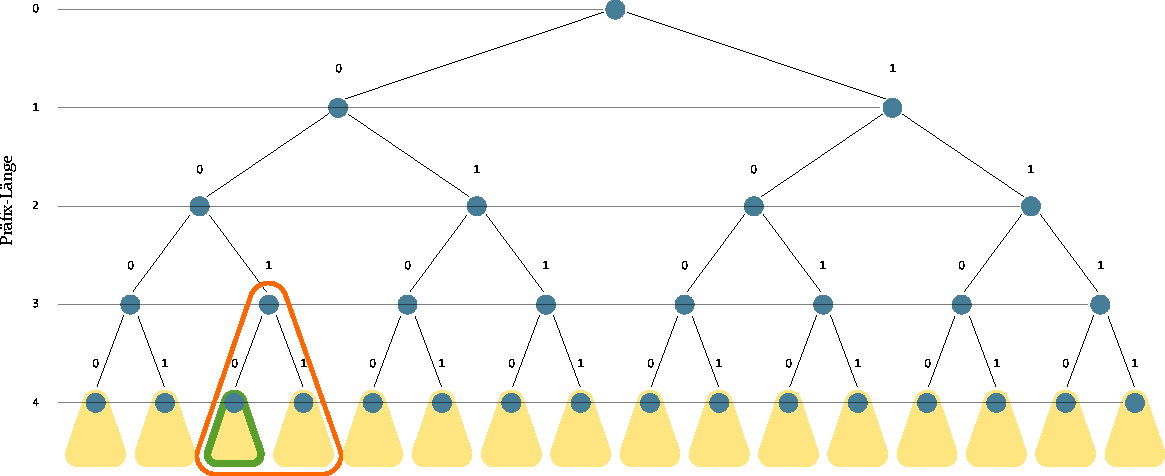
\includegraphics[width=\textwidth]{images/prefix-filter-binary-tree.pdf}
  \caption[Präfix-Filter: Binärbaum]{Die Pefix-Länge geht bis 64, jedes der gelben Dreiecke stellt folglich einen Teilbaum der Höhe 61 dar.}
  \label{fig:bintree}
  \end{figure}

  Anstelle von Streams stellen wir uns eine Adresse als Blatt eines Binärbaums der Höhe 65 vor. Die Position wird über die ersten 64 Bits des Ripe einer Adresse bestimmt. Eine Präfix-Lenge $n$ definiert den Teilbaum, ab welchem wir Meldungen lesen. Ein sendender Client setzt ein 64-Bit-Nonce, bei welchem die ersten $n$ Bits vom Ripe der Empfängeradresse kopiert und der Rest zufällig gesetzt wird.

  Nehmen wir nun an, der Ripe von Bobs Adresse starte mit \texttt{00101001\ldots} und hat eine Präfix-Länge von 3. Alice sendet ihre Meldung mit dem Tag \texttt{00110100\ldots}. Die ersten drei Bits müssen gleich sein, aber der Rest ist zufällig gewählt. Bobs Client verarbeitet nun alle Meldungen welche seinem Präfix entsprechen, er muss also nur \sfrac{1}{8} des Gesamttraffics lesen.\footnote{Im Moment ist der Traffic insgesamt etwa 1 GiB im Monat.}

  Wie Bitmessage populärer wird, wird es auch mehr und mehr Traffic generieren. Bob möchte deshalb möglicherweise seine Präfix-Länge auf 4 erhöhen, was den zu verarbeitenden Traffic weiter auf \sfrac{1}{16} des Gesamtvolumens reduziert. Um dies zu tun, publiziert er einfach seinen \obj{pubkey} mit seiner aktualisierten Präfix-Länge. Das heisst natürlich auch, dass entweder immer ein \obj{pubkey} publiziert sein muss, oder Alice muss wenigstens einmal online sein während der \obj{pubkey} publiziert ist. Andernfalls gibt es in unserem Szenario eine 50\% Chance dass die Nachricht Bob nicht erreicht.

  Die Methode der Präfix-Filterung würde es zwar einem Smartphone-Client erlauben nur seine eigenen Meldungen zu verarbeiten,\footnote{Ein Präfix von 64 würde höchstwahrscheinlich bedeuten dass man auf dem Stream nur seine eigenen Meldungen erhählt.} aber damit würde man auch seine Anonymität beinahe komplett aufgeben.

  \subsection{Forward Secrecy}

  Offensichtlich ist es für einen Angreifer trivial alle (verschlüsselten) Objekte zu sammeln, welche durch das Bitmessage-Netzwerk verteilt werden --- sofern Speicherplatz kein Problem ist. Sollte dieser Angreifer irgendwie an den privaten Schlüssel eines Benutzers kommen, kann er alle gespeicherten Meldungen entschlüsseln, welche für diesen Benutzer bestimmt sind, und sich ausserdem als diesen ausgeben.\footnote{Das Letztere ist schwieriger wenn der Schlüssel durch eine Bruteforce-Attacke erworben wurde.}

  Glaubhafte Abstreitbarkeit (plausible deniability) kann in einigen Szenarios dagegen helfen. Bei dieser Aktion --- auch "{}eine Adresse atomisieren"\footnote{"Nuking an address."} genannt --- wird der private Schlüssel anonym veröffentlicht.\footnote{Siehe \url{https://bitmessage.ch/nuked/} für ein Beispiel.}

  Perfect Forward Secrecy scheint nicht praktikabel implementierbar zu sein, da man dazu vor dem Senden der eigentlichen Nachricht Informationen austauschen muss. Dies braucht wiederum Proof of Work um das Netzwerk zu schützen, was für den Sender die doppelte Arbeit bedeutet und die dreifache Zeit eine Nachricht zu senden --- falls beide Clients online sind. Der Austausch von Nachrichten würde so gut wie unmöglich wenn beide Benutzer nur sporadisch online sind.

  \subsection{Mobile Client}

  Es gibt zwar inzwischen einen Client für Android,\footnote{Bitseal: \url{https://play.google.com/store/apps/details?id=com.github.bitseal}} dieser benötigt jedoch sehr viel Traffic, der Proof of Work dauert ewig und die Batterie hält nicht sehr lange.

  In PyBitmessage gibt es die Option, den Empfänger eindeutig identifizierbar zu machen. Dies würde es einem Server erlauben nur die relevanten Meldungen weiterzuleiten. Zwar gibt man dabei seine Anonymität auf, aber das ist immer noch besser als die Ansätze der E-Mail-Relays, wo der private Schlüssel gleich beim Server liegt.

  Ein Ansatz, der Anonymität trotz unterstützendem Server erlaubt, schlug Dan Smith vor.\cite{forum:msg7871} Dabei wird ein drittes Schlüsselpaar generiert, mit dem der String "{}IDENTIFICATION"{} und einige zufällige Bytes verschlüsselt wird. Der Relay-Server muss dabei den privaten Identifikationsschlüssel erhalten --- soweit muss man ihm also noch vertrauen. Wenn er also mit Hilfe des Identifikationsschlüssels den Text "{}IDENTIFICATION"{} extrahieren kann, ist die Meldung für mich bestimmt und wird weitergeleitet.

  Der Proof of Work schliesslich lässt sich sehr einfach auf einem Server erledigen. Mit einer optimierten Implementation sollte er aber auch auf einem modernen Smartphone in vernünftiger Zeit machbar sein. Die Geräte haben inzwischen oftmals mehr als vier Prozessorkerne und einen dedizierten Grafikchip, der sich ausgezeichnet zum parallelen Berechnen von Hashes eignet.

  \newpage
  \section{Diskussion}

  Anonymität hat ihren Preis. Bei Bitmessage ist es Traffic, Speicherplatz und Rechenpower. Bei E-Mail ist es Vertrauen. Wenn wir unserem E-Mail-Provider nicht vertrauen können (wer kann das?), ist Bitmessage eine Alternative, wenn auch nicht vollständig ausgereift.

  Ich finde die Idee eines Trustless-Protokolls\footnote{Ein Protokoll, das kein Vertrauen benötigt.} und Peer-To-Peer Netzwerke, die üblicherweise soche Protokolle verwenden, äusserst interessant. Zu Beginn war das Internet ein riesiges Netzwerk gleichberechtigter Teilnehmer, doch heutzutage scheint alles zu Google oder Facebook zu führen. P2P und Trustless-Protokolle geben uns ein Stück dieser Freiheit zurück, welche in der Cloud verlorengegangen ist.

  Dass es nun einen P2P E-Mail-Ersatz gibt finde ich absolut grossartig. Ja, es skaliert nicht so gut wie E-Mail. Aber dank Proof of Work denke ich, dass wir kein mit E-Mail vergleichbares Spam-Problem haben, was den Traffic schon mal gut halbiert. Falls Bitmessage E-Mail jemals ersetzt, würde ein grosser Teil des E-Mail-Verkehrs wohl eher durch Instant-Messaging ersetzt. Vor allem Firmenintern, wo eine eigene Infrastruktur aufgebaut werden kann, muss nicht unbedingt Bitmessage verwendet werden.

  \begin{figure}[htp]
  \centering
  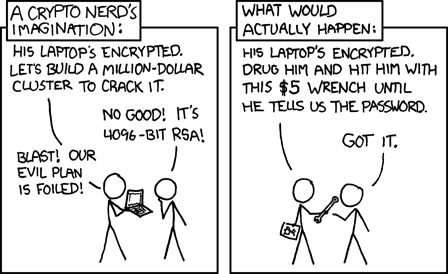
\includegraphics[width=0.7\textwidth]{images/xkcd-security.png}
  \caption[XKCD: Security]{\url{http://xkcd.com/538/}\nocite{xkcd:538}}
  \label{fig:xkcd}
  \end{figure}

  \newpage
  \bibliographystyle{plain}
  \bibliography{bibliography}
  \listoffigures

\end{document}